\section{Case Study}

Beyond theoretical explorations, our framework also supports practical modeling
distributed applications that may rely on complex combinations of semantics.
Instead of checking at source code level tracing possible code paths like Noctua
\cite{ma2024noctua} with SMT solvers, our approach operates at
axiomatic logic and
optionally application level, allowing researchers and system designers to
encode nodes (representing intermediate API endpoints or storage systems
providing consistency semantics) and edges (representing interactions or data
flows) within their systems. Each node may require or provide specific
consistency guarantees, while edges capture the ordering/visibility constraints
and optional application specific logics between events across services.

The \texttt{composable} function operates over a directed multigraph
whose nodes and
edges represent services (nodes) and interactions (edges) in a distributed
system. Each node and edge can specify which consistency guarantees it needs or
provides in the form of constraints (e.g., monotonic reads, read-your-writes).

\begin{itemize}
  \item \textit{Nodes:} each node represents a logical component like
    services or storage
    systems, each node can:
    \begin{itemize}
      \item Issue operations (e.g., read or write to shared state)
      \item Require certain consistency properties (e.g., monotonic
        reads) for these
        operations
      \item Provide certain consistency guarantees to downstream consumers
    \end{itemize}
    In the current implementation, each node stores:
    \begin{itemize}
      \item \texttt{name}: a unique identifier
      \item \texttt{needs}: a set of constraints that must be
        satisfied to uphold the node's
        required semantics
      \item \texttt{provs}: a set of constraints that characterize
        what the node provides to other
        nodes
    \end{itemize}

  \item \textit{Edges:} edges represent interactions or data flows
    between nodes, capturing:
    \begin{itemize}
      \item Precedence constraints (e.g., write `a` must return
        before read `b` starts) % Note: Consider \texttt{} for a and
        % b if they represent variables/values
      \item Required or optional additional constraints representing
        custom operations or
        relations that must hold between the source and destination nodes
    \end{itemize}
\end{itemize}

The \texttt{composable} function attempts to find an assignment of
constraints that
makes the entire graph "composable". In other words, it seeks a model in which
all nodes' \texttt{needs} can be matched with some nodes'
\texttt{provs}, and all edges'
constraints are satisfied simultaneously. This corresponds to verifying if there
is a coherent assignment of semantics across the system's interactions. Users
may provide zero or more semantics to \texttt{needs} and
\texttt{provs} for each node, and
similarly, zero or more constraints for each edge. During the check at each
level of the graph traversal, a \textit{pairwise} check between
source node \texttt{needs} in
conjunction of edge constraints against destination node
\texttt{provs} is performed.
If the pairwise check is successful, all previous assignments are recorded and
used as context for further checks. In case of pairwise check failure
(contradiction), the function backtracks and selects other possible assignments
if there are more than one provide in each of the source
\texttt{needs}, edge constraints, and destination \texttt{provs}.

% TODO: do we need pseudocode here?

\textit{Implementation:} given a starting node (conceptually, usually
a client) and a
set of premise constraints, the function begins a DFS through the graph. At each
node:
\begin{itemize}
  \item The function examines outgoing edges and their associated constraints.
  \item Each edge can impose conditions on the relationship between
    the source node's
    requirements (\texttt{needs}), the destination node's provided
    guarantees (\texttt{provs}),
    and any additional edge-specific constraints.
  \item The solver checks whether combining these constraints with
    the accumulated
    premise remains satisfiable.
\end{itemize}
If no consistent assignment is found for outgoing edges, the function
backtracks, exploring alternative paths or constraint combinations. During
traversal, the function uses the \texttt{compatible} checks behind
the scenes. For each
candidate combination of node-level and edge-level constraints, it
calls \texttt{compatible} to
ensure that no contradictions arise. If the DFS manages to visit all edges and
find consistent assignments for all node needs and provided constraints, the
function returns a \texttt{True} value along with a subgraph
(\texttt{result}) that records a
satisfying assignment. The returned subgraph shows which edges and nodes were
selected and how their constraints were matched. If no satisfying assignment is
found, the function returns \texttt{False}, and \texttt{None} for the graph.

% \subsection{Example: Online Shopping}
%
% Consider an online shop scenario where multiple services and
% components interact
% to process customer interactions and purchases. The shop maintains
% an inventory
% of products, and a shopping cart service, a transaction log to
% record purchases,
% and the the client itself. Additionally, an arbitrator node to coordinate
% interactions between the interactions between clients and the entire service
% stack.
%
% A customer uses a shopping cart service to preserve the state of
% the items they
% intend to buy. The customer can read or write the cart's contents, adjusting
% their intended purchases as they browse products. Let's say in this example,
% clients do not care to see their latest update to the cart being propagated to
% other devices immediately, but the states will eventually converge.
%
% The shop holds the canonical inventory state. Before finalizing a
% purchase, the
% customer's requested items must be checked against the shop's
% current inventory.
% If items are available, the transaction can proceed, if not, the request fails
% due to insufficient stock.
%
% Once the shop confirms inventory, it records the customer's purchase in the
% transaction log, and replicated across multiple nodes for fault tolerance.
%
% An arbitrator acts as a gatekeeper that serializes requests and interacts with
% both the shop (update inventory) and the transaction log
% (bookkeeping). When the
% customer decides to make a purchase, the arbitrator:
% \begin{itemize}
%   \item Receives requests from client and write to a intermediate
%     location (capturing
%     the customer's intent)
%   \item Reads from the shop's inventory to verify item availability
%   \item If available, writes back to the shop to decrement the
%     inventory and write and
%     replicate the transaction to the log
%   \item If not available, reply back to the client with an error
% \end{itemize}
%
% The arbitrator or serialization point pattern is commonly used in other system
% implementations like Paxos \cite{lamport2001paxos} to maintain a
% consistent order of
% events at critial locations, ensuring that purchase requests are
% applied to the
% shop and recorded in the transaction log in a well-defined sequence.
%
% \textit{Nodes:}
% \begin{itemize}
%   \item \textit{Arbitrator:} Provides linearizability
%   \item \textit{Tx:} Provides linearizability
%   \item \textit{Shop:} Provides RYW + MR, ensuring that once
%     arbitrator updates inventory, all
%     subsequent reads observe the writes
%   \item \textit{Client and Cart:} Represent endpoints that do not
%     enforce any semantic by
%     themselves but rely on the guarantees of the nodes they interact with
% \end{itemize}
%
% \textit{Edges:}
% \begin{itemize}
%   \item \texttt{Client} to \texttt{Cart} edge represent the customer
%     adding items to their cart
%   \item \texttt{Client} to \texttt{Shop} edge represent price checks
%     or Browse inventory
%   \item \texttt{Client} to \texttt{Arbitrator} edge represents a
%     purchase request
%   \item \texttt{Arbitrator} to \texttt{Shop} and \texttt{Arbitrator}
%     to \texttt{Tx} edges represent the arbitrator's
%     mediation: writing to the transaction log, reading and updating the shop's
%     inventory state in sequential order
% \end{itemize}
%
% In this example, the \texttt{composable} function succeeds with a
% graph containing one
% of the possible satisfiable constraint assignments.

{\color{purple}
  \subsection{Online Shopping System}

  We present a case study of an e-commerce application that
  demonstrates how our framework can model and verify consistency
  guarantees across multiple interacting services. This example
  illustrates a common pattern in distributed systems where different
  components require different consistency levels based on their
  functional requirements.

  \subsubsection{Architecture}

  The online shopping system consists of five key components that
  interact to provide a complete shopping experience:

  \begin{figure}[h]
    \centering
    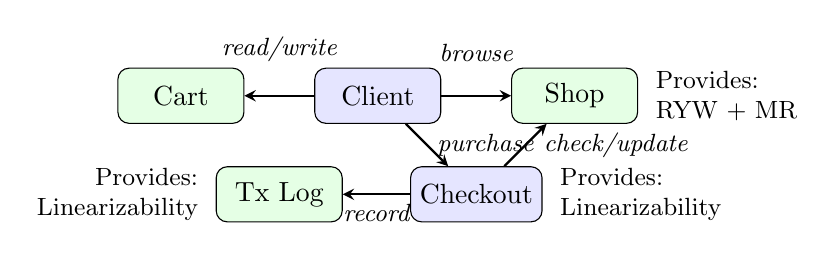
\begin{tikzpicture}[
        node distance=1.2cm,
        service/.style={draw, rounded corners, fill=blue!10, minimum
        width=1.6cm, minimum height=0.7cm},
        storage/.style={draw, rounded corners, fill=green!10, minimum
        width=1.6cm, minimum height=0.7cm},
        arrow/.style={->, >=stealth, thick},
        label/.style={font=\small\itshape}
      ]

      % nodes
      \node[service] (client) at (-0.3,0) {Client};
      \node[storage] (cart) at ([shift={(180:2.5cm)}]client) {Cart};
      \node[storage] (shop) at ([shift={(0:2.5cm)}]client) {Shop};
      \node[service] (arbitrator) at ([shift={(315:1.77cm)}]client)
      {Checkout};
      \node[storage] (tx) at ([shift={(225:1.77cm)}]client) {Tx Log};

      % edges
      \draw[arrow] (client) -- (cart) node[midway, above=0.3cm,
      label] {read/write};
      \draw[arrow] (client) -- (shop) node[midway, above=0.3cm, label] {browse};
      \draw[arrow] (client) -- (arbitrator) node[midway, right, label]
      {purchase};
      \draw[arrow] (arbitrator) -- (shop) node[pos=0.3175,
      right=0.2cm, yshift=0.1cm, label] {check/update};
      \draw[arrow] (arbitrator) -- (tx) node[midway, below, label] {record};

      % semantics
      \node[right=0.1cm, align=left, font=\small] at (shop.east)
      {Provides:\\RYW + MR};
      \node[right=0.1cm, align=left, font=\small] at (arbitrator.east)
      {Provides:\\Linearizability};
      \node[left=0.1cm, align=right, font=\small] at (tx.west)
      {Provides:\\Linearizability};
    \end{tikzpicture}
    \caption{Architecture of the online shopping system with
    consistency guarantees}
    \label{fig:case-study-shop}
  \end{figure}

  \begin{enumerate}
    \item \textbf{Client}: The end-user interface through which
      customers browse products, manage their shopping cart, and
      initiate purchases. The client itself doesn't enforce specific
      consistency guarantees but relies on the guarantees provided by
      the services it interacts with.

    \item \textbf{Cart}: The shopping cart service maintains customers
      shopping cart state. It stores items that customers intend to
      purchase and supports read and write operations. The cart service
      allows eventual convergence of state across multiple devices,
      meaning that immediate propagation of updates is not required.

    \item \textbf{Shop}: Maintains the authoritative inventory state
      for all products. The shop provides Read-Your-Writes (RYW) and
      Monotonic Reads (MR) guarantees, ensuring that once inventory is
      updated, all subsequent reads will observe these updates in a
      consistent manner. This combination allows for a balance between
      consistency and performance.

    \item \textbf{Arbitrator}: Acts as a serialization point for
      purchase transactions, providing linearizability guarantees. This
      critical component ensures that concurrent purchase requests are
      processed in a well-defined sequence, preventing race conditions
      that could lead to inventory inconsistencies or duplicate transactions.

    \item \textbf{Tx Log}: Records all completed purchases
      with linearizability guarantees, ensuring that transaction
      records are stored in a strictly consistent manner for auditing
      and financial reconciliation purposes.
  \end{enumerate}

  \subsubsection{Interaction Flow}

  The typical interaction flow in this system follows several patterns:

  \textbf{Browsing and Cart Management:} Customers interact directly
  with the shop service to browse available products. When they find
  items of interest, they can add these items to their cart through the
  cart service. These operations don't require strong consistency
  guarantees as they don't modify the authoritative inventory state.

  \textbf{Purchase Process:} When a customer decides to complete their
  purchase, a more complex interaction begins:

  \begin{enumerate}
    \item The client sends a purchase request to the arbitrator,
      including the contents of the customer's cart.

    \item The arbitrator, acting as a serialization point, first reads
      from the shop's inventory to verify that all requested items are
      available in sufficient quantities.

    \item If the inventory check succeeds, the arbitrator performs two
      operations in sequence:
      \begin{itemize}
        \item It writes to the shop service to decrement the inventory
          counts for the purchased items.
        \item It writes to the transaction log to record the successful
          purchase, capturing details such as items purchased,
          quantities, prices, and customer information.
      \end{itemize}

    \item If the inventory check fails (e.g., an item is out of stock),
      the arbitrator responds to the client with an error message, and
      no changes are made to either the inventory or transaction log.
  \end{enumerate}

  This interaction pattern ensures that inventory updates and
  transaction records are kept in sync, preventing scenarios where
  inventory is decremented without a corresponding transaction record
  or vice versa.

  \subsubsection{Requirements and Verification}

  The consistency requirements of this system vary by component:

  \begin{itemize}
    \item The shop service provides Read-Your-Writes and Monotonic
      Reads guarantees, which are sufficient for inventory management.
      RYW ensures that once the arbitrator updates inventory levels,
      any subsequent reads will observe these updates. MR ensures that
      if a client observes a certain inventory state, all subsequent
      reads will observe either that same state or a more recent one,
      preventing anomalies where inventory appears to increase without
      corresponding returns or restocking operations.

    \item The arbitrator and transaction log both provide
      linearizability, the strongest consistency model, ensuring that
      all operations appear to execute atomically in a sequential order
      that is consistent with the real-time ordering of those
      operations. This is critical for the financial aspects of the system.

    \item The cart service has more relaxed consistency requirements,
      as temporary inconsistencies in cart state don't impact the
      integrity of the inventory or financial records.
  \end{itemize}

  When we apply our \texttt{composable} function to this system,
  starting from the client node, it successfully verifies that the
  composition of these services with their respective consistency
  guarantees satisfies the overall system requirements. The function
  traverses the graph, checking at each step whether the constraints
  imposed by each node and edge are mutually satisfiable.

  The verification confirms that the arbitrator's linearizability
  guarantee is sufficient to coordinate between the shop's RYW+MR
  guarantees and the transaction log's linearizability, ensuring that
  inventory updates and transaction records remain consistent even
  under concurrent operations.
}

% TODO: rewrite with more detail like cross causal
% \subsection{Example: Streaming Service}
%
% Another example (simplified from DeathStarBench Media Service
% \cite{gan2019an}):
% consider a streaming service with multiple components handling user
% authentication, content delivery, and user interactions. The system comprises:
%
% \begin{itemize}
%   \item Admin: admin interface for content and user management operations
%   \item Client: end-user interface for accessing streaming content
% and features
%   \item Login: authentication service that acts like a user session manager
%   \item User DB: user credential storage
%   \item Metadata DB: content metadata storage
%   \item Rent: rental transaction service
%   \item Rent DB: transaction record storage
%   \item Review: user review service
%   \item Review DB: review storage
%   \item Video: video streaming service for content delivery
%   \item Video DB: video content storage providing
% \end{itemize}
%
% A user must first register and login through the authentication service before
% accessing any content. The login service verifies credentials against the User
% DB, which maintains consistent user states through Monotonic Writes and Writes
% Follow Reads guarantees as updates performed by users needs to be reflected to
% themselves right after.
%
% When Browse content, the client interacts with the metadata services. Before
% serving any content, users must first be authenticated through the login
% service, then clients can issue read to metadata database to retrieve titles.
% After selecting a media, clients can issue write to the Rent
% service to rent the
% media for viewing. The Rent service must ensure that the title is available
% through read to the metadata database. The Metadata DB provides
% Monotonic Reads
% and Read Your Writes guarantees, allowing admin updates to be
% reflected visible
% while tolerating some staleness for user reads.
%
% Users can also write reviews for content they've watched. The review service
% verifies content existence in Metadata DB. Writes the review to Review DB with
% Read-Your-Writes ensuring users see their own reviews immediately while other
% users may see slightly stale data.
%
% Administrators use a separate interface to manage content and user
% access. When
% uploading new content, the admin service updates metadata in Metadata DB,
% uploads video content to Video DB. Both operations require prior admin
% authentication (assuming admin users are pre-granted access). Video
% DB's Writes
% Follow Reads guarantee ensures content version consistency.
%
% As this example demonstrates, it's more complex than the online shopping mall
% example. Listing of nodes and edges is not exhaustive, please see the actual
% implementation for more details. The overall operational constraints are
% captured through custom operation types with quantified constraints optionally
% enforced at each node level.

\subsection{Media Streaming Service}

To demonstrate our framework's ability to model complex distributed
systems with diverse consistency requirements, we present a case
study of a media streaming service inspired by the DeathStarBench
Media Service benchmark. This example illustrates how our approach
\cite{gan2019an}
can verify the composition of multiple services with heterogeneous
consistency guarantees.

\subsubsection{System Architecture}

The media streaming service consists of eleven interconnected
components, each with specific consistency requirements based on
their functional roles:

\begin{figure}[h]
  \centering
  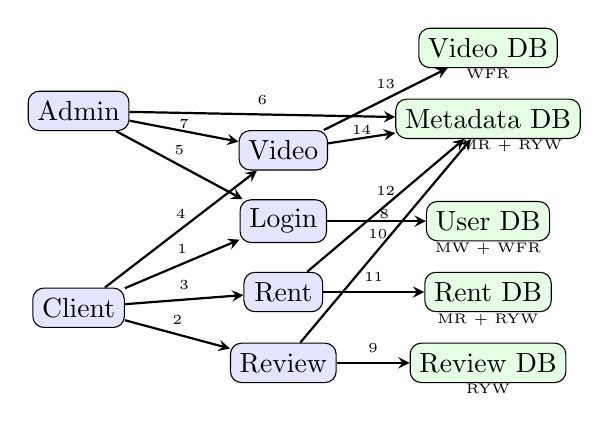
\begin{tikzpicture}[
      node distance=1.8cm,
      service/.style={draw, rounded corners, fill=blue!10, minimum
      width=1cm, minimum height=0.5cm},
      storage/.style={draw, rounded corners, fill=green!10, minimum
      width=1cm, minimum height=0.5cm},
      arrow/.style={->, >=stealth, thick},
      label/.style={font=\small\itshape}
    ]
    % client and admin
    \node[service] (client) at (0,0) {Client};
    \node[service, yshift=3mm] (admin) at (0,2.2) {Admin};

    % services
    \node[service] (login) at (2.6,1.1) {Login};
    \node[service] (review) at (2.6,-0.7) {Review};
    \node[service] (rent) at (2.6,0.2) {Rent};
    \node[service] (video) at (2.6,2.0) {Video};

    % db nodes
    \node[storage] (user_db) at (5.2,1.1) {User DB};
    \node[storage] (metadata_db) at (5.2,2.4) {Metadata DB};
    \node[storage] (review_db) at (5.2,-0.7) {Review DB};
    \node[storage] (rent_db) at (5.2,0.2) {Rent DB};
    \node[storage] (video_db) at (5.2,3.3) {Video DB};

    % edges from client with centered, above labels
    \draw[arrow] (client) -- (login) node[pos=0.5, above, font=\tiny] {1};
    \draw[arrow] (client) -- (review) node[pos=0.5, above, font=\tiny] {2};
    \draw[arrow] (client) -- (rent) node[pos=0.5, above, font=\tiny] {3};
    \draw[arrow] (client) -- (video) node[pos=0.5, above, font=\tiny] {4};

    % edges from admin
    \draw[arrow] (admin) -- (login) node[pos=0.5, above, font=\tiny] {5};
    \draw[arrow] (admin) -- (metadata_db) node[pos=0.5, above, font=\tiny] {6};
    \draw[arrow] (admin) -- (video) node[pos=0.5, above, yshift=-1mm,
    font=\tiny] {7};

    % service to DB edges
    \draw[arrow] (login) -- (user_db) node[pos=0.5, above,
    xshift=1mm, yshift=-1mm, font=\tiny] {8};
    \draw[arrow] (review) -- (review_db) node[pos=0.5, above, font=\tiny] {9};
    \draw[arrow] (review) -- (metadata_db) node[pos=0.5, above,
    xshift=-1mm, yshift=-1mm, font=\tiny] {10};
    \draw[arrow] (rent) -- (rent_db) node[pos=0.5, above, font=\tiny] {11};
    \draw[arrow] (rent) -- (metadata_db) node[pos=0.5, above, font=\tiny] {12};
    \draw[arrow] (video) -- (video_db) node[pos=0.5, above, font=\tiny] {13};
    \draw[arrow] (video) -- (metadata_db) node[pos=0.5, above,
    yshift=-0.8mm, font=\tiny] {14};

    % semantics for databases only
    \node[below=0.15cm, align=center, font=\tiny] at (user_db) {MW + WFR};
    \node[below=0.15cm, align=center, xshift=3mm, font=\tiny] at
    (metadata_db) {MR + RYW};
    \node[below=0.15cm, align=center, font=\tiny] at (review_db) {RYW};
    \node[below=0.15cm, align=center, font=\tiny] at (rent_db) {MR + RYW};
    \node[below=0.15cm, align=center, font=\tiny] at (video_db) {WFR};
  \end{tikzpicture}
  \caption{Architecture of the media streaming service with
    consistency guarantees.
    Edges are numbered for reference:
    1–4: Client requests to services (login, review, rent, video).
    5: Admin login.
    6: Admin updates metadata.
    7: Admin uploads video.
    8: Login service accesses User DB.
    9: Review service writes to Review DB.
    10: Review checks content existence in Metadata DB.
    11: Rent updates Rent DB.
    12: Rent checks content availability in Metadata DB.
    13: Video service accesses Video DB.
  14: Video service verifies metadata before playback.}
  \label{fig:case-study-media}
\end{figure}

\begin{enumerate}
  \item \textbf{Client and Admin}: These components represent the
    entry points for regular users and administrative personnel,
    respectively. They don't enforce specific consistency guarantees
    themselves but rely on the guarantees provided by the services
    they interact with.

  \item \textbf{Authentication}:
    \begin{itemize}
      \item \textbf{Login Service}: Manages user authentication and
        session handling. It requires Monotonic Writes (MW) and
        Writes Follow Reads (WFR) guarantees to ensure that user
        credential updates are properly sequenced and visible.
      \item \textbf{User Database}: Stores user credentials and
        profile information with MW and WFR guarantees. This ensures
        that when users update their profiles or credentials, these
        changes are consistently visible to subsequent operations.
    \end{itemize}

  \item \textbf{Content Management}:
    \begin{itemize}
      \item \textbf{Metadata Database}: Stores information about
        available media content (titles, descriptions, genres, etc.)
        with Monotonic Reads (MR) and Read Your Writes (RYW)
        guarantees. This allows administrative updates to be
        immediately visible while tolerating some staleness for user reads.
      \item \textbf{Video Service}: Handles video streaming requests
        and requires MR guarantees to ensure consistent content delivery.
      \item \textbf{Video Database}: Stores the actual video content
        with WFR guarantees to maintain version consistency.
    \end{itemize}

  \item \textbf{API}:
    \begin{itemize}
      \item \textbf{Review Service}: Manages user reviews and
        requires RYW guarantees to ensure users can immediately see
        their own reviews.
      \item \textbf{Review Database}: Stores user reviews with RYW
        guarantees, allowing users to see their own reviews
        immediately while other users might see slightly stale data.
      \item \textbf{Rent Service}: Handles media rental transactions
        and requires MR guarantees to ensure consistent inventory checks.
      \item \textbf{Rent Database}: Records rental transactions with
        MR and RYW guarantees to maintain consistent transaction history.
    \end{itemize}
\end{enumerate}

{\color{red}
  In this example, we've specified that all users must register for
  an account before they can log in, this would result in a request from
  client, to login service, then to user database.
  If users are to post a review, they must
  be logged in, and the review service must verify that the title exists
  in the metadata database before allowing the review to be written. This would
  incur the review service to validate user authentication status, then
  the existence of the title in the metadata database before writing
  to the review database. This is one of the clear dependency chains
  in the media service example.
  This dependency chain creates a cascading effect throughout the system
  where each operation builds upon the successful completion of its
  prerequisites.
  The registration-before-login dependency establishes user identity,
  the login-before-content-access dependency establishes authorization,
  and the content-validation-before-review dependency establishes
  referential integrity.

  Semantically, 6 nodes are interacting with each other (client,
    login service, user database, review service, metadata database,
  and review database).
  The edges between these nodes represent the flow of data and we
  encode the prerequisites
  of each operation as constraints on the edges. Implementation-wise,
  all constraints on edges can be
  directly encoded on the nodes themselves along with the
  aforementioned semantics. However, when modeling
  services with complex interactions with cross storage system
  dependencies, edge constraints can clearly
  separate the providing/requiring semantic constraints and
  downstream implementation specific
  service logic. In the implementation, we defined multiple operations
  with read or write type to represent interactions between nodes on the edge.
  For the registration operation, we simply abstract it as a write,
  and login operation as a read, and assign constraints to the operations.
  Formally, we can represent client's login operation as follow:

  \begin{align*}
    EC_{login} &\triangleq \forall op_{login} \in H_{rd} : \exists
    op_{reg} \in H_{wr} :\\
  &ob(op_{login}, op_{reg}) \land vis(op_{reg}, op_{login}))
\end{align*}

For services initiated from the client side, we modeled the behaviors
as a set of constraints with the return-before binary relationship. Formally:

\begin{align*}
  EC_{auth} &\triangleq rb(op_{login}, op_{rdreview}) \land
  rb(op_{login}, op_{wrreview}) \\
  &\land rb(op_{login}, op_{rent}) \land rb(op_{login}, op_{watch})
\end{align*}

These constraints are then added to each edge that's relevant to the
login service or refer to the login operation, ensuring the chain
of dependencies is respected throughout the system. For posting reviews,
the review service must first verify that the content exists in the
metadata database before allowing the review to be written. Similar to
the login operation, we can represent the review service's interaction
as a set of constraints with existential quantification, object constraints,
and return-before relationships, on top of consistency semantics
ended at each nodes'
provide and need fields.

% TODO: add review service constraints
}

\subsubsection{Interaction Flows}

The media streaming service supports several interaction patterns,
each with specific consistency requirements:

\textbf{User Registration and Authentication}: Before accessing any
content, users must register and authenticate through the login
service. This process involves:

\begin{enumerate}
\item The client sends a registration request (abstracted as a
  write operation) to the login service.
\item The login service writes the new user credentials to the User Database.
\item For subsequent logins, the client sends a login request
  (abstracted as a read operation) to the login service.
\item The login service reads from the User Database to verify credentials.
\end{enumerate}

The MW and WFR guarantees of the User Database ensure that once user
credentials are updated, all subsequent authentication attempts will
see the updated information, preventing authentication anomalies
where users might be unable to log in with newly created or changed credentials.

\textbf{Browsing and Playback}: Once authenticated, users can browse
and watch available content:

\begin{enumerate}
\item The client sends a request to browse content, which queries
  the Metadata Database.
\item When a user selects content to watch, the client sends a
  request to the Video Service.
\item The Video Service verifies the content's existence and
  availability by reading from the Metadata Database.
\item If the content is available, the Video Service streams the
  content from the Video Database to the client.
\end{enumerate}

The MR guarantee of the Video Service ensures that once a piece of
content is determined to be available, subsequent read operations
will maintain this view, preventing inconsistencies during playback.
The WFR guarantee of the Video Database ensures that if the service
reads a specific version of content, subsequent writes will not
revert to an earlier version.

\textbf{Rentals}: For premium content, users must first rent the content:

\begin{enumerate}
\item The client sends a rental request to the Rent Service.
\item The Rent Service checks content availability by reading from
  the Metadata Database.
\item If available, the Rent Service records the transaction in the
  Rent Database.
\item The client can then access the rented content through the Video Service.
\end{enumerate}

The MR guarantee of the Rent Service ensures consistent inventory
checks, preventing scenarios where content appears to be available
and then becomes unavailable during the rental process.

\textbf{Reviews}: Users can read and write reviews for content they've watched:

\begin{enumerate}
\item To read reviews, the client sends a request to the Review
  Service, which retrieves reviews from the Review Database.
\item To write a review, the client sends the review content to the
  Review Service.
\item The Review Service verifies that the content exists by
  reading from the Metadata Database.
\item If verified, the Review Service writes the review to the
  Review Database.
\end{enumerate}

The RYW guarantee of both the Review Service and Review Database
ensures that users immediately see their own reviews after
submission, providing a responsive user experience while allowing for
eventual consistency for other users' views.

\textbf{Admin Operations}: Administrators manage content through
separate workflows:

\begin{enumerate}
\item Administrators authenticate through the Login Service (with
  pre-granted access).
\item To add new content, administrators:
  \begin{itemize}
    \item Upload video content to the Video Database through the
      Video Service.
    \item Add corresponding metadata to the Metadata Database.
  \end{itemize}
\item To modify user accounts, administrators interact with the
  Login Service, which updates the User Database.
\end{enumerate}

The combination of RYW and MR guarantees in the Metadata Database
ensures that administrative updates are immediately visible to the
administrators themselves while allowing for controlled propagation
to user-facing services.

\subsubsection{Requirements and Verification}

Each component in the system has specific consistency requirements
based on its functional role:

\begin{itemize}
\item The User Database provides MW and WFR guarantees, ensuring
  that credential updates are properly sequenced and visible, which
  is critical for authentication security.

\item The Metadata Database provides MR and RYW guarantees,
  balancing immediate visibility of administrative updates with
  tolerance for some staleness in user reads.

\item The Review Database provides RYW guarantees, prioritizing the
  user experience of seeing one's own reviews immediately while
  accepting eventual consistency for other users' views.

\item The Rent Database provides MR and RYW guarantees, ensuring
  consistent transaction records for both administrative and user views.

\item The Video Database provides WFR guarantees, maintaining
  version consistency for content delivery.
\end{itemize}

The edges in our model represent not just data flow but also critical
operational constraints. For example, the edge from the Client to the
Login Service carries the constraint that "User must register before
login," enforced through a visibility relationship between
registration and login operations. Similarly, the edge from the
Review Service to the Metadata Database enforces the constraint that
"Check metadata before read review," ensuring that reviews are only
accessible for valid content.

When we apply \texttt{composable} function to this system,
starting from the client node, it successfully verifies that the
composition of these services with their respective consistency
guarantees satisfies the overall system requirements. The function
traverses the graph, checking at each step whether the constraints
imposed by each node and edge are mutually satisfiable.

This verification confirms that despite the heterogeneous consistency
guarantees across different components, the system as a whole
maintains its required properties. For instance, the login flow
correctly enforces that registration must precede login, and the
review system correctly ensures that users can immediately see their
own reviews while maintaining content validity checks.

% \subsection{Example: Antipode \cite{ferreira2023antipode}}
% TODO: rewrite after wrapping up
% Basic encodings of lineage and cross-service causal consistency (XCY) are
% finished but full implementation is still in progress. See
% \texttt{tests/test\_antipode.py} for
% details.

\subsection{Example: Cross Service Causal}

When reading the graph, think of it as a reversed tree (rooted from svc1) with
one branch growing from root to leaf (xc). The leaf node's (xc) prov/need field
in the implementation is set to \texttt{None} to indicate that it
does not provide any
guarantees, and will only be used for extraction (see descriptions below).
Implementation of \texttt{tests/test\_cross\_causal.py}:

\begin{verbatim}
            xc
           / <- mr + mw + ryw
        svc4 - wfr
       / <- mr + mw + wfr
     svc3 - ryw
    / <- mr + ryw + wfr
  svc2 - mw
 / <- mw + ryw + wfr
svc1 - mr
\end{verbatim}

This example demonstrates modeling a system where multiple services, each
offering only a basic consistency guarantee, are chained together. The goal is
to verify if their composition, mediated by specific inter-service constraints,
symbolic isolation, and the role of explicit ``glue'' constraints.

\textit{Setup}\footnote{I decided not to use the ``pseudo node'' in
the write up, it makes the explanation unnecessarily complex.}: We
model a linear chain of services: $\text{SVC1} \rightarrow
\text{SVC2} \rightarrow \text{SVC3} \rightarrow \text{SVC4}
\rightarrow \text{XC}$.
Each service $\text{SVC}n$ (for $n=1..4$) is designed to provide only
\textit{one} of the
four session guarantees via its \texttt{provs} attribute:
$\text{SVC}1$ provides MR, $\text{SVC}2$ provides
MW, $\text{SVC}3$ provides RYW, and $\text{SVC}4$ provides WFR.

\textit{Symbolic Isolation:} To prevent logical interference, the
guarantee provided by
each service (e.g., \texttt{MonotonicReads.assertions}) and the
constraints added on
the edges are instantiated using unique symbols specific to that service or edge
(e.g., using helpers like \texttt{gensym} and \texttt{assertion\_for}
from \texttt{tests/test\_cross\_causal.py}).
This ensures, for example, that the Monotonic Reads constraints of
$\text{SVC}1$ only
apply to operations symbolically designated as belonging to $\text{SVC}1$.

\textit{Composition via Edge Constraints:} The composition logic
resides in the ``glue''
constraints defined on the \texttt{cons} attribute of the edges connecting the
services. Since each service node only provides one session
guarantee, the edge $\text{SVC}n \rightarrow \text{SVC}(n+1)$ must
provide constraints representing the other three session guarantees needed to
potentially satisfy Causal Consistency up to that point.

The core idea of this example is to build a stronger guarantee by composing
weaker guarantees provided by individual services ($\text{SVC}1
\ldots 4$), using the
edges to supply the missing pieces. Verbatim:

\begin{itemize}
\item $\text{SVC}1$ starts by providing only MR (via its
  \texttt{provs}, using symbols like $a_1, b_1, \ldots$).
  Its own \texttt{needs} are \texttt{None}.
\item To potentially achieve Causal Consistency for operations
  passing from $\text{SVC}1$ to $\text{SVC}2$,
  the edge $\text{Edge}(\text{SVC1} \rightarrow \text{SVC2})$ must
  provide the other three required
  session guarantees: MW, RYW, and WFR (via its \texttt{cons},
  using unique symbols like $a_{12}, b_{12}, \ldots$).
  However, in real world implementations, edge constraints usually requires
  additional application specific logic to be satisfiable. In other word, edge
  constraints used in abstract representation implies the existence
  of application
  level protocols that enforces convergence of data either through
  consensus (like
  Raft \cite{diego2014raft} or Paxos \cite{lamport1998paxos}) or other means.
\item When \texttt{composable} evaluates this step, it checks if
  the interaction is locally
  consistent based on the nodes' defined
  \texttt{provs}/\texttt{needs} and the edge's \texttt{cons}. If
  this local check passes (meaning $\text{SVC}2$'s required guarantee, Causal
    Consistency, is satisfied through what the edge + $\text{SVC}1$'s
  provs provide), we
  \textit{interpret} this (based on our setup) as achieving Causal
  Consistency for the
  combined path ($\text{SVC}1 + \text{Edge}(\text{SVC1} \rightarrow
  \text{SVC2})$) leading \textit{up to} $\text{SVC}2$.
\item Now, although the path leading to $\text{SVC}2$ is causally
  consistent, $\text{SVC}2$ itself,
  according to its definition in this example, only
  \textit{provides} MW to the outside
  world (via its \texttt{provs}, using symbols $a_2, b_2, \ldots$).
\item Therefore, for the \textit{next} service, $\text{SVC}3$, to
  maintain Causal Consistency
  relative to the operations flowing through the
  ($\text{SVC}1\rightarrow\text{SVC}2$) mesh, the edge
  $\text{Edge}(\text{SVC2} \rightarrow \text{SVC3})$ must
  supply the guarantees missing relative to $\text{SVC}2$'s
  provided MW. This means $\text{Edge}(\text{SVC2} \rightarrow
  \text{SVC3})$ must
  provide MR, RYW, and WFR (again, with unique symbols).
\item This pattern repeats: each service node $\text{SVC}n$
  provides one specific
  guarantee, and the edge $\text{Edge}(n \rightarrow n+1)$ provides
  the complementary guarantees
  needed to ensure the cumulative path maintains the target property.
\end{itemize}

\textit{Symbol Equivalence:} For this composition to be meaningful, we must
conceptually link operations across services that refer to the same logical
action or data. For instance, if write $a_1$ in $\text{SVC}1$ and
write $a_2$ in $\text{SVC}2$ both
represent updates to the same user profile, ``glue'' constraints
equating relevant
aspects (like $a_1.\text{obj} = a_2.\text{obj}$ or $a_1.\text{ival} =
a_2.\text{ival}$ despite their
different symbolic names) might be necessary. While the current test
code (\texttt{tests/test\_cross\_causal.py})
simplifies this by focusing on composing the consistency axioms, a more rigorous
model would include these explicit symbol equivalence constraints on the edges
(we are directly asserting symbols of $a_1$ are identical of those of $a_2$ for
simplicity).

\textit{Aggregation:} The \texttt{composable(g, svc1)} call attempts
to find a satisfying
assignment for the entire chain, respecting the \texttt{provs} of
each node and the \texttt{cons} of
each edge. If it returns \texttt{True}, it confirms that the
individual guarantees can
be composed under the specified edge constraints. Subsequently,
\texttt{extract(svc1, svc1, (ok, res))} can
synthesize a single logical formula representing the net end-to-end guarantee
achieved by the chain, starting from $\text{SVC}1$. This aggregated
constraint (\texttt{aggcons} in
the test code) could then be compared against a formal definition of Causal
Consistency.
